\documentclass[journal,12pt,twocolumn]{IEEEtran}

\usepackage{setspace}
\usepackage{gensymb}
\singlespacing
\usepackage[cmex10]{amsmath}

\usepackage{amsthm}

\usepackage{mathrsfs}
\usepackage{txfonts}
\usepackage{stfloats}
\usepackage{bm}
\usepackage{cite}
\usepackage{cases}
\usepackage{subfig}

\usepackage{longtable}
\usepackage{multirow}

\usepackage{enumitem}
\usepackage{mathtools}
\usepackage{steinmetz}
\usepackage{tikz}
\usepackage{circuitikz}
\usepackage{verbatim}
\usepackage{tfrupee}
\usepackage[breaklinks=true]{hyperref}
\usepackage{graphicx}
\usepackage{tkz-euclide}

\usetikzlibrary{calc,math}
\usepackage{listings}
    \usepackage{color}                                            %%
    \usepackage{array}                                            %%
    \usepackage{longtable}                                        %%
    \usepackage{calc}                                             %%
    \usepackage{multirow}                                         %%
    \usepackage{hhline}                                           %%
    \usepackage{ifthen}                                           %%
    \usepackage{lscape}     
\usepackage{multicol}
\usepackage{chngcntr}

\DeclareMathOperator*{\Res}{Res}

\renewcommand\thesection{\arabic{section}}
\renewcommand\thesubsection{\thesection.\arabic{subsection}}
\renewcommand\thesubsubsection{\thesubsection.\arabic{subsubsection}}

\renewcommand\thesectiondis{\arabic{section}}
\renewcommand\thesubsectiondis{\thesectiondis.\arabic{subsection}}
\renewcommand\thesubsubsectiondis{\thesubsectiondis.\arabic{subsubsection}}


\hyphenation{op-tical net-works semi-conduc-tor}
\def\inputGnumericTable{}                                 %%

\lstset{
%language=C,
frame=single, 
breaklines=true,
columns=fullflexible
}
\begin{document}


\newtheorem{theorem}{Theorem}[section]
\newtheorem{problem}{Problem}
\newtheorem{proposition}{Proposition}[section]
\newtheorem{lemma}{Lemma}[section]
\newtheorem{corollary}[theorem]{Corollary}
\newtheorem{example}{Example}[section]
\newtheorem{definition}[problem]{Definition}

\newcommand{\BEQA}{\begin{eqnarray}}
\newcommand{\EEQA}{\end{eqnarray}}
\newcommand{\define}{\stackrel{\triangle}{=}}
\bibliographystyle{IEEEtran}
\raggedbottom
\setlength{\parindent}{0pt}
\providecommand{\mbf}{\mathbf}
\providecommand{\pr}[1]{\ensuremath{\Pr\left(#1\right)}}
\providecommand{\qfunc}[1]{\ensuremath{Q\left(#1\right)}}
\providecommand{\sbrak}[1]{\ensuremath{{}\left[#1\right]}}
\providecommand{\lsbrak}[1]{\ensuremath{{}\left[#1\right.}}
\providecommand{\rsbrak}[1]{\ensuremath{{}\left.#1\right]}}
\providecommand{\brak}[1]{\ensuremath{\left(#1\right)}}
\providecommand{\lbrak}[1]{\ensuremath{\left(#1\right.}}
\providecommand{\rbrak}[1]{\ensuremath{\left.#1\right)}}
\providecommand{\cbrak}[1]{\ensuremath{\left\{#1\right\}}}
\providecommand{\lcbrak}[1]{\ensuremath{\left\{#1\right.}}
\providecommand{\rcbrak}[1]{\ensuremath{\left.#1\right\}}}
\theoremstyle{remark}
\newtheorem{rem}{Remark}
\newcommand{\sgn}{\mathop{\mathrm{sgn}}}
\providecommand{\abs}[1]{\left\vert#1\right\vert}
\providecommand{\res}[1]{\Res\displaylimits_{#1}} 
\providecommand{\norm}[1]{\left\lVert#1\right\rVert}
%\providecommand{\norm}[1]{\lVert#1\rVert}
\providecommand{\mtx}[1]{\mathbf{#1}}
\providecommand{\mean}[1]{E\left[ #1 \right]}
\providecommand{\fourier}{\overset{\mathcal{F}}{ \rightleftharpoons}}
%\providecommand{\hilbert}{\overset{\mathcal{H}}{ \rightleftharpoons}}
\providecommand{\system}{\overset{\mathcal{H}}{ \longleftrightarrow}}
\providecommand{\ztrans}{\overset{\mathcal{Z}}{ \rightleftharpoons}}
	%\newcommand{\solution}[2]{\textbf{Solution:}{#1}}
\newcommand{\solution}{\noindent \textbf{Solution: }}
\newcommand{\cosec}{\,\text{cosec}\,}
\providecommand{\dec}[2]{\ensuremath{\overset{#1}{\underset{#2}{\gtrless}}}}
\newcommand{\myvec}[1]{\ensuremath{\begin{pmatrix}#1\end{pmatrix}}}
\newcommand{\mydet}[1]{\ensuremath{}}
\numberwithin{equation}{subsection}

\makeatletter
\@addtoreset{figure}{problem}
\makeatother
\let\StandardTheFigure\thefigure
\let\vec\mathbf

\renewcommand{\thefigure}{\theproblem}

\def\putbox#1#2#3{\makebox[0in][l]{\makebox[#1][l]{}\raisebox{\baselineskip}[0in][0in]{\raisebox{#2}[0in][0in]{#3}}}}
     \def\rightbox#1{\makebox[0in][r]{#1}}
     \def\centbox#1{\makebox[0in]{#1}}
     \def\topbox#1{\raisebox{-\baselineskip}[0in][0in]{#1}}
     \def\midbox#1{\raisebox{-0.5\baselineskip}[0in][0in]{#1}}
\vspace{3cm}
\title{Quiz 2}
\author{Tanmay Goyal - AI20BTECH11021}
\maketitle
\newpage
\bigskip
\renewcommand{\thefigure}{\theenumi}
\renewcommand{\thetable}{\theenumi}

Download all latex codes from 
\begin{lstlisting}
https://github.com/tanmaygoyal258/EE3900-Linear-Systems-and-Signal-processing/blob/main/Quiz2/main.tex
\end{lstlisting}
\begin{lstlisting}
https://github.com/tanmaygoyal258/EE3900-Linear-Systems-and-Signal-processing/blob/main/Quiz2/code.py
\end{lstlisting}
\section{Problem}
(Oppenheim/3.24(a)) Sketch the following sequence and determine its z-transform, including its region of convergence:
\begin{align}
    a[n] = \sum_{k = -\infty}^\infty \delta[n-4k]
\end{align}
\section{Solution}
\begin{lemma}
\begin{align}
x(t) \times \delta(t-t_1) = x(t_1) \times \delta(t-t_1)
\label{multiplication}
\end{align}
\end{lemma}
\begin{proof}
\begin{align}
\delta(t-t_1) = 
\begin{cases}
0 & t \neq t_1\\
\infty & t=t_1
\end{cases}\\
\implies x(t) \times \delta(t-t_1) = 
\begin{cases}
0 & t \neq t_1\\
x(t_1) \times \infty & t=t_1
\end{cases}\\
 = x(t_1) \times \begin{cases}
0 & t \neq t_1\\
\infty & t=t_1
\end{cases}\\
 = x(t_1)\times \delta(t-t_1)
\end{align}

\end{proof}
The Z-transform of a signal $x[n]$ is given by:
\begin{align}
    x[n] \ztrans X(z) = \sum_{n = -\infty}^\infty x[n] z^{-n}
\end{align}
Thus, the z-transform of $a[n]$ is given by:
\begin{align}
    A(z) = \sum_{n = -\infty}^\infty a[n] z^{-n}\\
     = \sum_{n = -\infty}^\infty \sum_{k = -\infty}^\infty \delta[n-4k] z^{-n}\\
      = \sum_{k = -\infty}^\infty\sum_{n = -\infty}^\infty\delta[n-4k] z^{-n}\\
       = \sum_{k = -\infty}^\infty\sum_{n = -\infty}^\infty\delta[n-4k] z^{-4k}
\end{align}
using \eqref{multiplication}. Thus, we get:
\begin{align}
    A(z) =  \sum_{k = -\infty}^\infty z^{-4k}\sum_{n = -\infty}^\infty\delta[n-4k] \\ 
    = \sum_{k = -\infty}^\infty z^{-4k}
\end{align}
using the fact that:
\begin{align}
    \sum_{n = -\infty}^\infty \delta[n-m] = 1
\end{align}
When $k > 0$, the term $z^{-4k}$ becomes undefined for $z = 0$, and similarly when $k < 0$, the term $z^{-4k}$ is undefined when $z = \pm\infty$. Thus, the region of convergence is:
\begin{align}
    ROC = z \in \mathbb{R} \setminus \{0 , \pm\infty\}
\end{align}

\begin{figure}[!ht]
\centering
 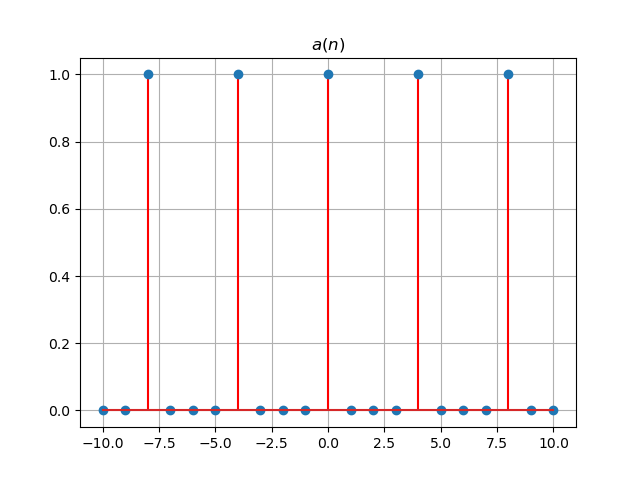
\includegraphics[width=\columnwidth]{Graphs/a.png}
 \caption{$a[n]$}
 \end{figure}
 \begin{figure}[!ht]
\centering
 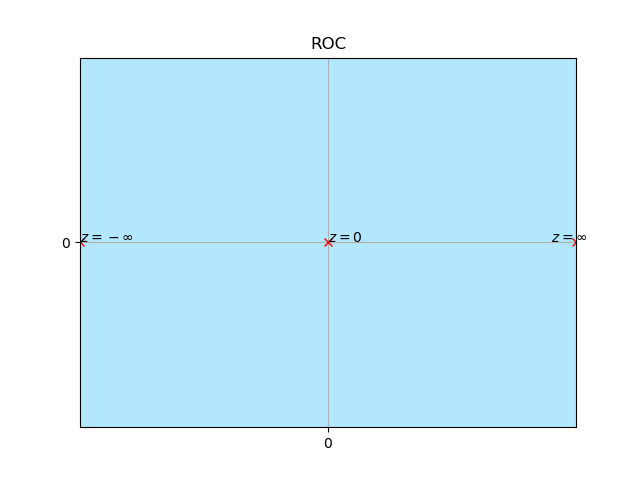
\includegraphics[width=\columnwidth]{Graphs/ROC.png}
 \caption{ROC}
 \end{figure}

\end{document}